% Proposed components A/B and training-only pair constraints C.
% Real observed inputs and training representatives; features/paths remain schematic.
\begin{tikzpicture}[x=1cm,y=1cm,font=\sffamily\fontsize{8.5}{10}\selectfont,text=ink,
 flow/.style={-{Latex[length=2.9pt,width=2.2pt]},draw=ink!58,line width=.7pt,line cap=round,line join=round},
 obsflow/.style={flow,draw=obsblue,line width=.85pt},
 actflow/.style={flow,draw=dynorange,line width=.85pt},
 pair/.style={<->,>=Latex,dashed,line width=.85pt},
 shell/.style={draw=ink!22,fill=white,rounded corners=2pt,line width=.5pt,inner sep=0pt},
 badge/.style={circle,minimum size=.43cm,inner sep=0pt,text=white,font=\sffamily\bfseries\fontsize{8.5}{10}\selectfont},
 title/.style={font=\sffamily\bfseries\fontsize{9.5}{11}\selectfont},
 code/.style={circle,minimum size=.68cm,inner sep=0pt,line width=.8pt}]
\path[use as bounding box] (0,-.70) rectangle (14,11.30);
\node[title] at (2.06,10.96) {Observed inputs};
\node[badge,fill=obsblue] at (5.84,10.96) {A};
\node[title,anchor=west,text=obsblue] at (6.13,10.96) {Shared calibration};
\node[badge,fill=dynorange] at (10.08,10.96) {B};
\node[title,anchor=west,text=dynorange] at (10.36,10.96) {Dynamics inference};

% Deployment input examples. The entire support filmstrip owns the output port.
\node at (3.20,10.13) {Goal $o_g$};
\node[shell,minimum width=1.31cm,minimum height=1.31cm] (goal) at (3.20,9.13) {};
\node[inner sep=0pt] at (3.20,9.13) {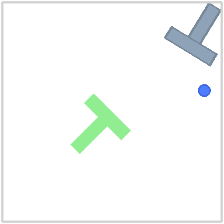
\includegraphics[width=1.20cm]{figures/assets/method_pusht_frame_7.png}};
\node at (2.06,8.15) {Observed history $o_S$};
\fill[ink!5,rounded corners=2pt] (.45,6.48) rectangle (3.90,7.87);
\node[shell,minimum width=3.55cm,minimum height=1.30cm] (history) at (2.08,7.23) {};
\foreach \idx/\xx in {0/.93,1/2.08,2/3.23}{
 \node[inner sep=0pt] at (\xx,7.23) {\includegraphics[width=1.10cm]{figures/assets/method_pusht_frame_\idx.png}};
}
\foreach \yy/\tag in {9.13/goal,7.23/history}{
 \node[shell,fill=ink!3,minimum width=.57cm,minimum height=.65cm] (enc\tag) at (4.42,\yy) {$E_0$};
 \node[inner sep=0pt] at (4.42,\yy+.52) {
\includegraphics[width=.20cm]{figures/assets/material_lock.png}};
}
\draw[flow] (goal.east) -- (encgoal.west);
\draw[flow] (history.east) -- (enchistory.west);

% A: one visibly shared channel-wise affine map of goal and support features.
\fill[obsblue!12,rounded corners=3pt] (5.92,6.58) rectangle (8.33,9.74);
\draw[fill=obsblue!3,draw=obsblue!55,line width=.85pt,rounded corners=3pt]
 (5.85,6.64) rectangle (8.25,9.80);
\node[text=obsblue,font=\fontsize{15}{17}\selectfont] at (7.05,8.39) {$A_o$};
\node[text=obsblue] at (7.05,8.01) {scale + shift};
\foreach \yy/\offset in {9.13/0,7.23/.07}{
 \fill[white,rounded corners=1.3pt] (5.97,\yy-.38) rectangle (8.12,\yy+.38);
 \foreach \xin/\xout/\hh/\scale/\shift/\shade in {
  6.05/7.42/.18/1.08/.12/35,6.22/7.59/.44/.94/-.05/60,
  6.39/7.76/.30/1.06/.13/43,6.56/7.93/.53/.96/-.08/73}{
  \pgfmathsetmacro{\beforeHeight}{\hh-\offset}
  \pgfmathsetmacro{\afterHeight}{\scale*\beforeHeight+\shift}
  \fill[ink!\shade] (\xin,\yy-.27) rectangle ++(.115,\beforeHeight);
  \fill[obsblue!\shade] (\xout,\yy-.27) rectangle ++(.115,\afterHeight);
 }
 \node[text=obsblue,font=\fontsize{12}{14}\selectfont] at (7.05,\yy) {$\times\!+$};
}
\draw[flow] (encgoal.east) -- (5.85,9.13);
\draw[flow] (enchistory.east) -- (5.85,7.23);
\node at (5.14,9.42) {$u_g$};
\node at (5.14,7.53) {$u_S$};
\node[shell,draw=obsblue!55,fill=obsblue!4,minimum width=2.40cm,minimum height=.66cm]
 (obsinfer) at (7.05,6.09) {};
\node[text=obsblue] at (6.36,6.09) {$\mu,\sigma^2$};
\draw[obsflow] (6.88,6.09) -- (7.38,6.09);
\node[text=obsblue,font=\fontsize{12}{14}\selectfont] at (7.80,6.09) {$c_o$};
\draw[flow] (5.25,7.23) -- (5.25,6.09) -- (obsinfer.west);
\fill[ink!60] (5.25,7.23) circle[radius=.026];
\draw[obsflow] (obsinfer.north) -- (7.05,6.64);
\node[text=obsblue] at (7.05,10.25) {same $A_o$, same $c_o$};

% B: chronological corrected transitions and actual executed actions.
\node at (11.68,10.15) {Executed $a_S$};
\node[shell,draw=dynorange!35,fill=dynorange!3,minimum width=1.55cm,minimum height=.42cm]
 (executed) at (11.68,9.66) {};
\draw[actflow] (11.11,9.66) -- (11.48,9.66);
\draw[actflow] (11.86,9.57) -- (12.23,9.75);
\node[shell,draw=dynorange!60,fill=dynorange!3,minimum width=3.45cm,minimum height=1.32cm]
 (dyninfer) at (11.73,7.49) {};
\foreach \xx/\shade in {10.23/45,10.38/65,10.98/55,11.13/80}{
 \fill[obsblue!\shade] (\xx,7.00) rectangle ++(.10,.42);
}
\draw[obsflow] (10.61,7.22) -- (10.86,7.22);
\node[text=obsblue] at (10.75,7.81) {$z_t,\Delta z_t$};
\node[shell,draw=dynorange!45,minimum width=.72cm,minimum height=.48cm] (gru) at (12.00,7.23) {GRU};
\draw[flow] (11.35,7.23) -- (gru.west);
\node[text=dynorange,font=\fontsize{12}{14}\selectfont] (cd) at (13.02,7.23) {$c_d$};
\draw[actflow] (gru.east) -- (cd.west);
\draw[actflow] (executed.south) -- (11.68,8.85) -- (12.00,8.85) -- (gru.north);
\draw[obsflow] (8.25,7.23) -- (10.00,7.23);
\node[text=obsblue] at (8.91,7.53) {$z_S$};
\fill[obsblue] (8.78,7.23) circle[radius=.027];

% Conventional planning is quiet gray; each candidate yields latent futures.
\node[shell,fill=ink!3,minimum width=.76cm,minimum height=.73cm] (predictor) at (9.20,5.12) {$P$};
\node[shell,fill=dynorange!3,draw=dynorange!40,minimum width=1.11cm,minimum height=.73cm]
 (ad) at (10.85,5.12) {$A_d\circ E_a$};
\node[shell,fill=ink!2,minimum width=1.74cm,minimum height=.73cm] (candidates) at (12.65,5.12) {};
\foreach \xx in {12.15,12.65,13.15}{
 \draw[draw=ink!30,rounded corners=1pt] (\xx-.20,4.96) rectangle (\xx+.20,5.28);
 \draw[flow] (\xx-.13,5.12) -- (\xx+.13,5.12);
}
\node at (12.52,5.77) {candidates};
\node[text=ink!65] at (9.20,4.59) {LeWM};
\draw[obsflow] (8.78,7.23) -- (8.78,6.48) -- (9.20,6.48) -- (predictor.north);
\draw[actflow] (cd.south) -- (13.02,6.48) -- (10.85,6.48) -- (ad.north);
\draw[flow] (candidates.west) -- (ad.east);
\draw[flow] (ad.west) -- (predictor.east);

% Three schematic latent sequences. The outlined left token is terminal.
% No pixel predictions, measured candidate scores, or winning candidate implied.
\node[shell,fill=ink!1,minimum width=2.03cm,minimum height=1.29cm]
 (futures) at (7.50,4.99) {};
\node at (7.50,5.42) {Latent futures};
\foreach \yy/\shade in {5.06/40,4.80/55,4.54/70}{
 \foreach \xx/\step in {8.06/0,7.51/1,6.96/2}{
  \draw[draw=ink!35,fill=white,rounded corners=.4pt,line width=.45pt]
   (\xx-.16,\yy-.09) rectangle (\xx+.16,\yy+.09);
  \foreach \dx/\ht/\phase in {-.10/.07/0,-.025/.11/70,.05/.05/145}{
   \pgfmathsetmacro{\schematicHeight}{\ht+.025*sin(55*\step+\phase+\shade)}
   \fill[ink!\shade] (\xx+\dx,\yy-.055) rectangle ++(.04,\schematicHeight);
  }
 }
 \draw[flow,line width=.5pt,-{Latex[length=1.8pt,width=1.4pt]}] (7.88,\yy) -- (7.69,\yy);
 \draw[flow,line width=.5pt,-{Latex[length=1.8pt,width=1.4pt]}] (7.33,\yy) -- (7.14,\yy);
 \draw[draw=ink!75,line width=.75pt,rounded corners=.5pt]
  (6.78,\yy-.11) rectangle (7.14,\yy+.11);
}
\draw[flow] (predictor.west) -- (8.515,5.12);
\node[shell,fill=ink!3,minimum width=1.25cm,minimum height=.96cm]
 (goalmse) at (5.25,5.12) {};
\node at (5.25,5.35) {MSE};
% Terminal prediction and common goal are visibly compared in feature space.
\foreach \xx/\tone in {4.87/ink,5.40/obsblue}{
 \foreach \dx/\hh in {0/.16,.08/.23,.16/.12}{
  \fill[\tone!65] (\xx+\dx,4.80) rectangle ++(.045,\hh);
 }
}
\node at (5.21,4.91) {$-$};
\draw[flow] (6.485,5.12) -- (goalmse.east);
\node[text=ink!65] at (6.18,5.43) {$\hat z_H^i$};
\node[shell,fill=ink!3,minimum width=1.43cm,minimum height=.96cm] (cem) at (3.40,5.12) {};
\node at (3.40,5.35) {CEM};
\node at (3.40,4.94) {$\mu,\sigma$};
\draw[flow] (goalmse.west) -- (cem.east);
\node at (4.37,5.42) {$J_i$};
\node[text=ink!65] at (2.38,4.38) {elite refit};
\node[shell,draw=dynorange,fill=dynorange!6,minimum width=.57cm,minimum height=.38cm] (first) at (1.17,5.12) {};
\draw[actflow] (.98,5.12) -- (1.36,5.12);
\node at (1.17,5.77) {first block};
\draw[flow] (cem.west) -- (first.east);
\node at (1.86,5.43) {mean plan};
\draw[actflow] (first.west) -- (.12,5.12) -- (.12,7.23) -- (history.west);
\node[text=ink!65] at (2.16,6.08) {act $\to$ observe};

% CEM resamples actions; the loop never represents a weight update.
\draw[flow] (cem.south) -- (3.40,3.70) -- (12.65,3.70) -- (candidates.south);
\node[text=ink!65] at (9.36,3.94) {resample action plans};
% Goal wire has an explicit bridge over the independent resampling route.
% The single continuous blue path receives a local white bridge under-stroke.
\draw[white,line width=3.1pt] (12.83,4.16) arc[start angle=0,end angle=180,radius=.18];
\draw[obsflow] (8.25,9.13) -- (8.78,9.13) -- (8.78,10.49) -- (13.76,10.49)
 -- (13.76,4.16) -- (12.83,4.16) arc[start angle=0,end angle=180,radius=.18]
 -- (5.25,4.16) -- (goalmse.south);
\node[text=obsblue] at (9.45,10.21) {$z_g$};
\node[text=obsblue] at (5.68,4.38) {goal};

% C is an OFFLINE relation panel, not additional deployment information.
\begin{scope}[yshift=-.70cm]
\draw[dashed,draw=ink!35,fill=ink!1,rounded corners=3pt,line width=.65pt]
 (.16,.16) rectangle (13.78,4.22);
\node[badge,fill=ink] at (.61,3.91) {C};
\node[title,anchor=west] at (.93,3.91) {Paired context supervision};
\node[anchor=east,text=ink!70] at (13.42,3.91) {training only; off in Unpaired contexts};
\node[title,text=dynorange] at (3.48,3.35) {Same trajectory, different appearances};
\node[title,text=obsblue] at (10.40,3.35) {Same appearance, batch $i\ne j$};
\draw[ink!18,line width=.5pt] (6.86,.43) -- (6.86,3.10);
% Representative clips: preserved real training frame on a temporal stack.
\foreach \yy/\vv in {2.50/0,.98/1}{
 \draw[fill=white,draw=ink!20,rounded corners=1pt] (.80,\yy-.46) rectangle (1.99,\yy+.67);
 \draw[fill=white,draw=ink!25,rounded corners=1pt] (.75,\yy-.51) rectangle (1.94,\yy+.62);
 \node[inner sep=0pt] at (1.29,\yy) {\includegraphics[width=1.10cm]{figures/split_assets/pusht_v\vv.png}};
 \node at (.43,\yy) {$v_\vv$};
 \node[shell,draw=dynorange!45,minimum width=1.18cm,minimum height=.58cm] (ab\vv) at (3.09,\yy) {A $\to$ B};
 \draw[flow] (1.88,\yy) -- (ab\vv.west);
 \node[text=ink!65] at (2.17,\yy+.26) {$E_0$};
 \node[code,draw=dynorange,fill=dynorange!5] (dc\vv) at (4.78,\yy) {$c_d^{v_\vv}$};
 \draw[flow] (ab\vv.east) -- (dc\vv.west);
}
\node[shell,draw=dynorange!30,fill=dynorange!3,minimum width=.68cm,minimum height=.30cm]
 (sharedacts) at (3.09,1.76) {};
\draw[actflow] (2.87,1.76) -- (3.31,1.76);
\node at (2.37,1.76) {$a_S$};
\draw[actflow] (sharedacts.north) -- (ab0.south);
\draw[actflow] (sharedacts.south) -- (ab1.north);
\draw[pair,draw=dynorange] (dc0.south) -- (dc1.north);
\node[text=dynorange,font=\fontsize{12}{14}\selectfont] at (5.54,1.76) {$\mathcal L_d$};
% Different minibatch entries; shared appearance does not mean matched state.
\foreach \yy/\tag/\which in {2.50/i/0,.98/j/1}{
 \draw[fill=white,draw=ink!20,rounded corners=1pt] (7.75,\yy-.46) rectangle (8.94,\yy+.67);
 \draw[fill=white,draw=ink!25,rounded corners=1pt] (7.70,\yy-.51) rectangle (8.89,\yy+.62);
 \ifnum\which=0
  \node[inner sep=0pt] at (8.24,\yy) {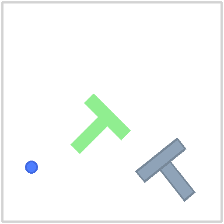
\includegraphics[width=1.10cm]{figures/split_assets/pusht_v0.png}};
 \else
  \node[inner sep=0pt] at (8.24,\yy) {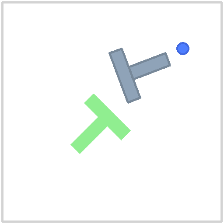
\includegraphics[width=1.10cm]{figures/assets/method_train_other.png}};
 \fi
 \node at (7.37,\yy) {$v_0$};
 \node[shell,draw=obsblue!50,minimum width=1.08cm,minimum height=.58cm] (ocmap\tag) at (10.02,\yy) {$C_o$};
 \draw[flow] (8.84,\yy) -- (ocmap\tag.west);
 \node[text=ink!65] at (9.15,\yy+.26) {$E_0$};
 \node[code,draw=obsblue,fill=obsblue!5] (oc\tag) at (11.71,\yy) {$c_o^{\tag}$};
 \draw[flow] (ocmap\tag.east) -- (oc\tag.west);
}
\draw[pair,draw=obsblue] (oci.south) -- (ocj.north);
\node[text=obsblue,font=\fontsize{12}{14}\selectfont] at (12.47,1.76) {$\mathcal L_o$};
\end{scope}
\end{tikzpicture}
